\section{Core concepts}\label{sec:core-concepts}

In this section, we discuss the integral core concepts of continuous integration
in order to give the reader a good understanding of its principles.

\subsection{Motivation}\label{sec:motivation}

The main goal of continuous integration is to minimize integration issues when
deploying release-versions of the product. Because builds happen often and
regularly, these issues can be identified very quickly and will not cause
stressful last-minute fixes. The incorporation of unit tests into the
build (see \ref{sec:tests}) can further increase fast error detection.

\subsubsection{Merge hell}

In big software projects, a large number of developers work together to create
software. To be able to work on the same project simultaneously, typically, a
version-control system such as GIT is utilized
\footnote{\url{http://git-scm.com/}}.\\

Developers usually branch off from a common baseline ("master"), implement their
feature in their own copy ("feature-branch") and when finished, merge their
branch back into the master. However, if a large number of developers do that,
and their features are large and/or implemented in overlapping parts of the
source code, developers have to face merge-conflicts when integrating their
branch back into the baseline. These conflicts can easily get out of hand.
Figure \ref{fig:merge-hell} shows an example of such a situation.

\begin{figure}[h]
    \centering
    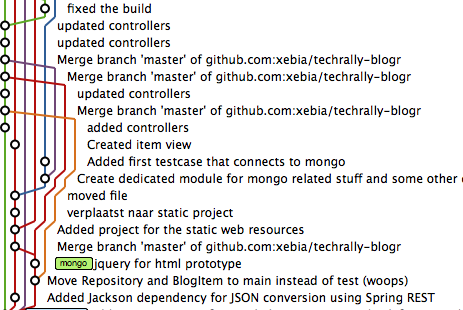
\includegraphics[width=0.6\linewidth]{images/merge-hell.png}
    \caption{An example of "merge-hell" \cite{mooij:2010}}
    \label{fig:merge-hell}
\end{figure}

Solving these conflicts can be non-trivial task, especially for the introduction
of completely new features, since the developer who has to perform the merge
typically is not yet accustomed to the code another developer only just
created.\\

In order to keep large merge conflicts to a minimum and therefore circumvent
this issue, continuous integration strives to integrate features back into the
baseline branch frequently (e.g. multiple times per day).  Of course, this means
that the term "feature" is bound to refer only to small changes throughout the
project's life cycle.

\subsubsection{Triggers}\label{sec:triggers}

\subsubsection{Builds}\label{sec:builds}

\subsubsection{Tests}\label{sec:tests}

Best practice: Test in clone of real production...

\subsubsection{Static code analysis}\label{sec:static-code-analysis}

\subsubsection{Deployment}\label{sec:deployment}

\paragraph{Migrations}\label{sec:migrations}

\subsection{Source control}\label{sec:source-control}

\subsection{Reporting}\label{sec:reporting}

